\documentclass[hyp,12pt]{socreport}

% Some generic packets.
\usepackage{color, colortbl}
\usepackage{url}
\usepackage{graphicx}
\usepackage{caption}
\usepackage{subcaption}
\usepackage{pgfplots}
\usepackage{tabularx}
\usepackage{multirow}
\usepackage{listings}
\pgfplotsset{width=10cm,compat=1.9}

% Sets the root path to look for all images.
\graphicspath{{images/}}

% Sets default options for listings.
\renewcommand\lstlistlistingname{List of Listings}
\newcommand*\lstinputpath[1]{\lstset{inputpath=#1}}
\lstinputpath{listings}
\lstset{frame=single, tabsize=2, captionpos=b}


\begin{document}
\pagenumbering{roman}

% Replace as necessary
\title{An Example HYP Final Report}
\author{Harold Finch}
\projyear{2015}
\projnumber{123-45-6789}
\advisor{Dr. Samaritan}
\deliverables{
    \item Report: 1 Volume
}
\maketitle

% Replace as necessary
\begin{abstract}
This report demonstrates the format of the SOC HYP final report and acts as boilerplate.

\begin{descriptors}
\item Networks
    \begin{itemize}
    \item[] Network protocols
        \begin{itemize}
        \item[] Application layer protocols
            \begin{itemize}
            \item[] Peer-to-peer protocols
            \end{itemize}
        \end{itemize}
    \end{itemize}
    \item[] Network services
        \begin{itemize}
        \item[] Programmable networks
        \end{itemize}
\end{descriptors}
\begin{keywords}
    Keyword 1, Keyword 2, Keyword 3
\end{keywords}

% Replace/Delete as necessary
\begin{implement}
    LaTeX, Mac OSX 10.10.2
\end{implement}


\end{abstract}

% Replace as necessary
\begin{acknowledgement}
See \texttt{README.md} of this repository.
\end{acknowledgement}

\listoffigures % Remove if no figures
\listoftables % Remove if no tables
\lstlistoflistings % Remove if no listings
\tableofcontents

% Actual contents in the contents folder.
% Include additional tex files here.
\chapter{Introduction}
This is the introduction of the example report using LaTex\cite{lamport1986document}. Also an example citation.

\section{Goals}
This is some \textbf{BOLD} text.

This is some \textit{italicised} text.

This is some \texttt{monospaced} text.

This is some math: $a^2 + b^2 = c^2$.

\subsection{Contributions}
This is an example of an enumeration.

\begin{enumerate}
    \item Point one.
    \item Point two.
    \item Point three.
\end{enumerate}

\begin{lstlisting}[
    language=TeX,
    caption={Example Listing.}
]
\title{An Example HYP Final Report}
\author{Harold Finch}
\projyear{2015}
\projnumber{123-45-6789}
\advisor{Dr. Samaritan}
\deliverables{
    \item Report: 1 Volume
}
\maketitle
\end{lstlisting}
\chapter{Results}
REPLACE WITH ACTUAL CONTENTS.

\section{Section 1}

\begin{table}[h]
\centering
\begin{tabular}{|l|l|l|l|}
\hline
         & Scissors & Paper & Stone \\ \hline
Scissors & Draw     & Win   & Lose  \\ \hline
Paper    & Lose     & Draw  & Win   \\ \hline
Stone    & Win      & Lose  & Draw  \\ \hline
\end{tabular}
\caption{Rules for Scissors-Paper-Stone.}
\label{table:example}
\end{table}

Table~\ref{table:example} shows an example table.

\section{Section 2}

\begin{figure}[h]
\centering
\begin{subfigure}[b]{.5\textwidth}
  \centering
  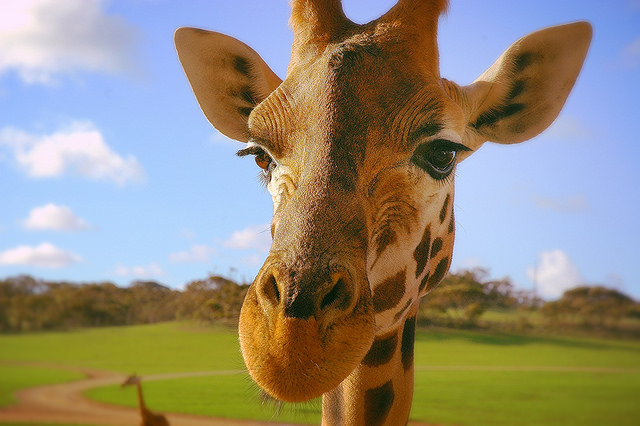
\includegraphics[width=.5\linewidth]{giraffe.jpg}
  \caption{An adorable Giraffe.}
\end{subfigure}%
\begin{subfigure}[b]{.5\textwidth}
  \centering
  
\includegraphics[width=.5\linewidth]{squirrel.jpg}
  \caption{An adorable Squirrel.}
\end{subfigure}
\caption{Adorable Animals.\label{fig:example}}
\end{figure}

In Figure~\ref{fig:example}, we have an example of images as sub-figures. Also animals.
\chapter{Conclusion}

Hopefully this example report is helpful.

\section{Section 1}

\subsection{Sub Section 1}

Some text here.

\subsection{Sub Section 2}

Moar text here.

\section{Section 2}

Fin.

\bibliographystyle{socreport}
\bibliography{report}

% Appendix (Remove if no appendix)
\appendix
\chapter{First appendix}
blah blah
\chapter{Second appendix}
blah blah

\end{document}
